\documentclass[conference,letterpaper]{IEEEtran}
\usepackage[T1]{fontenc}
\usepackage{newtxtext,newtxmath}
\usepackage{graphicx,booktabs,url}
\usepackage[hidelinks]{hyperref}
\usepackage{tikz}
\usetikzlibrary{positioning,arrows.meta}
\title{Better Vercel for Immutable Static Web Previews on AWS}
% Add verified author, affiliation, and email information here before submission.
% \author{\IEEEauthorblockN{Author Name}\IEEEauthorblockA{Department and Institution\\City, Country\\email@example.com}}
\begin{document}
\maketitle
\begin{abstract}
Static web previews require more than object upload: a deployment service must bind artifacts to projects, preserve deployment identity across retries, validate completed uploads, and route browser requests without masking missing assets. This paper presents Better Vercel, a prototype that separates local or GitHub Actions builds from an AWS control plane and a CloudFront delivery plane. The implementation combines a private Amazon S3 bucket, manifest-bound presigned uploads, conditional DynamoDB state transitions, a command-line client, and a web dashboard. Static exports and opt-in single-page applications use distinct storage namespaces. Evaluation comprises 86 passing local tests and retained live verification records from the Mumbai region. Two three-file Vite fixtures reached readiness 1.983 s and 1.240 s after build completion; these are individual smoke-test observations, not latency distributions. Live checks cover project-token isolation, checksum enforcement, overwrite rejection, interrupted-upload recovery, concurrent finalization, and routing behavior. The results support feasibility for trusted, temporary previews. Shared browser origins, visibility before finalization, incomplete hosted-build acceptance, and unverified long-term costs remain limitations.
\end{abstract}
\begin{IEEEkeywords}
static web hosting, serverless computing, immutable deployments, Amazon Web Services, deployment verification
\end{IEEEkeywords}
\section{Introduction}
A static deployment platform connects build output to a stable preview URL. Although serving HTML, JavaScript, and CSS is straightforward, the surrounding workflow must address partial uploads, repeated requests, concurrent finalization, incorrect asset paths, and authorization between projects. These concerns become visible when a prototype grows beyond a single operator copying files into an object store.

Better Vercel addresses this workflow through a deliberately limited system: builds execute on a developer machine or a GitHub Actions runner, while AWS stores validated artifacts and serves public previews. The implementation is a private alpha for trusted projects, with seven-day artifact retention. It does not provide server-side rendering, public signup, billing, production aliases, or automatic rollback \cite{r1}. The project name does not imply measured superiority over another hosting platform.

The engineering contribution is the integration of an immutable upload protocol, project-scoped request identity, explicit routing modes, and an evidence-based verification process. The study asks whether this design can preserve deployment identity during retries, reject invalid cross-project operations, and correctly serve small static and single-page application previews. It evaluates implemented behavior and recorded smoke tests rather than comparative performance or production availability.

\section{Technical Background and Scope}
Static export separates application compilation from request serving. For example, Next.js can produce HTML and supporting assets that a conventional static server can deliver, while features requiring a server are outside that export model \cite{r2}. Better Vercel therefore accepts generated assets rather than executing application code in its AWS serving path. Framework support depends on an application's output and configuration, not merely its framework label.

Amazon CloudFront origin access control provides authenticated access to an S3 origin \cite{r3}. In this system, it permits a private bucket to back public preview URLs. Origin privacy and viewer authorization are different properties: preventing direct anonymous S3 reads does not make CloudFront previews private. S3 conditional writes provide a separate primitive: an If-None-Match precondition can reject writes when an object already exists \cite{r4}. DynamoDB condition expressions similarly allow state updates only when their expected conditions hold \cite{r5}.

These established service mechanisms form the foundation of the prototype. The work is a systems integration study, not a new storage consistency algorithm. It combines the primitives with a manifest contract, deterministic deployment identity, framework-aware path configuration, and a CLI/dashboard workflow. No controlled comparison with managed hosting products is performed.

\section{System Architecture}
\begin{figure}[t]\centering
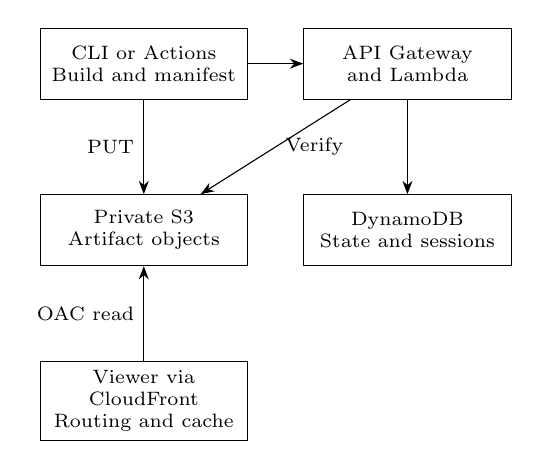
\begin{tikzpicture}[node distance=12mm and 7mm, every node/.style={font=\scriptsize}, box/.style={draw,align=center,text width=24mm,minimum height=9mm}, >=Stealth]
\node[box] (client) {CLI or Actions\\Build and manifest};
\node[box,right=of client] (api) {API Gateway\\and Lambda};
\node[box,below=of client] (s3) {Private S3\\Artifact objects};
\node[box,below=of api] (db) {DynamoDB\\State and sessions};
\node[box,below=of s3] (cdn) {Viewer via CloudFront\\Routing and cache};
\draw[->] (client) -- (api); \draw[->] (client) -- node[left]{PUT} (s3);
\draw[->] (api) -- (db); \draw[->] (api) -- node[right]{Verify} (s3);
\draw[->] (cdn) -- node[left]{OAC read} (s3);
\end{tikzpicture}
\caption{Build, control, and delivery paths. Artifact uploads go directly to S3; viewer requests do not consult deployment state.}\label{fig:architecture}
\end{figure}
\subsection{Build and Delivery Planes}
Figure 1 separates build execution, deployment coordination, and content delivery. The CLI executes only the configured build command, collects output, computes SHA-256 digests, and requests upload instructions. Static artifacts move directly from the client to S3 through individual presigned PUT URLs. Artifact bodies do not pass through Lambda. The serving path is CloudFront plus S3 and does not invoke the control API for each page request \cite{r1}.

The hosting stack uses an S3 bucket with public access blocked, bucket-owner-enforced ownership, server-side S3 encryption, and HTTPS enforcement. CloudFront redirects viewers to HTTPS and invokes a viewer-request function to map preview paths to storage keys. Its origin read grant is restricted to deployment and dashboard prefixes for the designated distribution. A separate dashboard behavior disables caching and applies restrictive response headers.

\subsection{Control Plane and Metadata}
The control stack contains an API Gateway HTTP API, one ARM64 Node.js 24 Lambda function, and three on-demand DynamoDB tables. The function has 256 MiB of memory and a 28 s timeout, runs outside a VPC, and has no provisioned concurrency. The API stage is configured for 5 requests/s with a burst limit of 10. These settings constrain normal operation but do not constitute a hard spending cap \cite{r1}.

The Projects table records project identity and salted token hashes. Deployments uses a project partition key and deployment sort key to store manifests, request hashes, state, timestamps, and bounded state logs. GitHubConnections stores session/setup records and ownership links; expiring records use a TTL attribute. All three tables are encrypted and retained on stack deletion. Deployment queries use strongly consistent reads and pagination; their descending deployment-ID order must not be interpreted as chronological ordering.

\subsection{Authentication and GitHub Integration}
Operator project creation requires AWS Signature Version 4 and IAM authorization. Normal CLI operations use project bearer tokens, whose server-side representations are salted scrypt hashes. A token authorizes only its owning project. Clients receive per-object signed URLs rather than AWS access keys. The Lambda role spans the application's project-artifact namespace, so cross-project authorization still depends on correct application checks and signing logic; it is not enforced by a distinct IAM principal for each project.

The optional GitHub flow uses authorization-code OAuth with PKCE, a fixed callback, single-use state, and server-side session validation, following GitHub's documented authorization mechanisms \cite{r6}. GitHub access tokens remain server-side; the dashboard holds an opaque session token in memory. The client secret is obtained from one permitted Secrets Manager ARN. Generated workflows pin a source commit and keep the deployment token out of dependency-installation and build-step environments. This separation reduces accidental exposure but is not a sandbox against malicious repository code. Imports are manual snapshots, not automatic deployments on every source push \cite{r1}.

\section{Deployment Protocol}
\subsection{Manifest Validation and Request Identity}
The manifest lists each relative path, byte length, content type, and SHA-256 digest. A nonempty root index.html is required. The API rejects traversal, absolute paths, duplicate paths, unsupported extensions, and mismatched MIME types. Its limits are 500 files, 25 MiB of total artifact content, and 220,000 bytes for the JSON body. These are independent limits: a manifest can satisfy the file-count limit yet exceed the request-body limit.

Deployment creation requires a project-scoped idempotency key. A normalized request hash includes artifact metadata, framework, routing mode, and supplied source metadata. File ordering does not change request identity. Repeating a key with the same request returns the existing deployment; changing the request returns a conflict. This allows an interrupted upload to resume without creating another deployment. The issued preview base path is supplied to the build so that generated links and assets refer to the correct deployment.

\subsection{Create-Only Uploads and Finalization}
A deployment has a 15 min upload window. Individual signed URLs last at most 5 min and do not outlive that window. Their instructions bind the object key, size, MIME type, cache policy, checksum, and create-only precondition. An explicit IAM deny prevents the API role from performing artifact PUT operations without the required If-None-Match value. Once an object exists, a repeated conditional upload is rejected; clients can skip previously uploaded files during recovery \cite{r1}, \cite{r4}.

Finalization compares the stored objects with the complete manifest, including exact keys, sizes, checksums, MIME types, and cache headers. Missing objects remain retryable; mismatches or expiry produce a failed deployment. Conditional DynamoDB transitions ensure that concurrent successful finalizers converge on one ready record and repeated finalization preserves its readiness timestamp. Ready is therefore a metadata statement that validation completed, not a transactional boundary that makes an entire directory visible atomically.

Known CloudFront object paths may be fetched before finalization because the delivery plane does not consult deployment state. Similarly, the implementation does not snapshot an entire object set in a single storage transaction. Its guarantees arise from create-only uploads, a bounded upload window, validation, and conditional metadata updates. Publication gating would require an additional design change.

\subsection{Routing and Framework Constraints}
Static previews use a public /d/<id>/ base and project-owned storage keys. Directory paths resolve to their index.html objects; extensionless paths are canonicalized to directory URLs. There is no global error-to-HTML fallback. Missing JavaScript, CSS, or unknown deployment paths therefore remain errors, including expected S3-origin 403 responses when callers cannot list the private bucket.

An explicit SPA mode adds /\_spa/ to the public base and uses a separate storage namespace within the project. Only paths with no dot fall back to the SPA root document. Dotted routes and asset paths remain exact requests. This avoids returning HTML for a missing script and prevents a static deployment's root document from being used as its SPA fallback. Dotted client-side route names are consequently unsupported by this fallback rule.

Next.js static exports require static routing, trailing-slash directory output, a deployment-specific base path, and unoptimized images. The prototype does not support SSR, API routes, middleware, server actions, ISR, or the default server-backed image optimizer. For SPA builds, absolute deployment-base asset URLs are required because relative HTML assets can break at nested history routes. The CLI's HTML path checks catch common mistakes but do not fully analyze CSS or runtime-generated URLs.

\subsection{Deletion and Retention}
Deletion is delayed until 16 min after creation, allowing the upload window and a safety margin to expire. It removes exact manifest keys and requests invalidation of both viewer and rewritten CloudFront paths. Clients repeat DELETE until the deployment reaches deleted; a read-only status request does not advance deletion. Metadata remains as a tombstone, preventing reuse of the immutable deployment identity.

There is no background deletion queue. Interrupted clients must resume deletion. Artifact lifecycle expiry is configured at seven days, incomplete multipart uploads at one day, and Lambda logs at three days. S3 lifecycle processing is asynchronous, and cached objects can remain available after origin removal until cache expiry or invalidation. Metadata may outlive content, so a retained ready record is not proof that a preview remains available indefinitely.

\section{Evaluation Methodology}
Evaluation combines a fresh local check of the source revision in \cite{r1} with previously retained live reports \cite{r7}. The local command npm run check performs TypeScript checking, bundles the API with its SDK dependencies, and runs the Node.js test suite. On October 24, 2026, all 86 tests passed, with no failures or skipped tests. The suite covers domain validation, storage adapters, CLI behavior, routing, infrastructure assertions, dashboard behavior, OAuth, repository detection, and workflow generation. Passing tests establish behavior for those cases; they are not a completeness proof or a live penetration test.

Live verification ran in AWS ap-south-1. Recorded timestamps on October 23 UTC correspond to October 24 in India Standard Time. The API verifier created two independent projects and exercised authorization in both directions, signed-prefix tampering, invalid artifacts, interrupted uploads, checksum and overwrite rejection, concurrent finalization, isolated listings, and preview-byte comparisons. The routing verifier deployed distinct static and SPA fixtures and checked MIME types, deep links, queries, missing assets, namespace isolation, and unknown deployments \cite{r7}.

Two timing boundaries are kept separate. Post-build readiness is measured from completion of the build callback until the CLI deployment operation returns. The routing script measures this before its subsequent HTTP content-verification loop. The earlier CLI smoke report instead records elapsed time including the build. Neither measure is browser load time, global CDN propagation time, nor a cold-start benchmark. Each row in Table I is one observation of its fixture, without repeated trials or controlled network conditions.

\section{Results and Discussion}
\begin{table}[t]\caption{Observed Deployment Times}\label{tab:results}\centering\footnotesize
\begin{tabular}{lrrrr}\toprule
Fixture & Files & Bytes & Time (s) & Boundary \\
\midrule
Vite SPA & 3 & 2,544 & 1.983 & Post-build \\
Vite static & 3 & 2,534 & 1.240 & Post-build \\
Vite CLI & 3 & 2,430 & 5.609 & With build \\
Next static & 19 & 398,084 & 16.004 & With build \\
\bottomrule\end{tabular}
\par\smallskip\raggedright One observation per fixture. Post-build timing excludes later HTTP content checks; with-build timing uses a different boundary. Source: \cite{r7}.
\end{table}
\subsection{Functional and Timing Results}
Table I reports the observed timings and exact artifact sizes. The SPA and static routing fixtures reached readiness in 1.983 s and 1.240 s after their builds, respectively, satisfying the verifier's 120 s post-build target for those runs. The two values do not establish that static routing is intrinsically faster: the experiment lacks repetition, randomized order, and control over service or network variability. The older Vite and Next.js observations include build time and must not be compared directly with the post-build values.

The retained API report lists ten passed check categories, including bidirectional token and signed-prefix isolation, checksum enforcement, immutable uploads, and duplicate/concurrent finalization. The separate routing completion record lists seven successful checks. An older pending label in the general API report still names SPA fallback; the dedicated routing report supplies the more specific completion evidence. This distinction avoids treating a stale checklist label as a failed routing test.

GitHub rollout evidence confirms enabled sign-in, CORS preflight, OAuth/PKCE redirects, rejection of a verifier mismatch, server-side secret retrieval with an intentionally invalid code exchange, protected repository endpoints, and matching dashboard assets. It does not establish a completed user-consent flow or a successful hosted Actions deployment. Local runner tests exercise plain HTML staging and a nested Vite build; actual hosted workflow execution remains a separate acceptance criterion \cite{r7}.

\subsection{Cost and Operational Interpretation}
The architecture avoids an always-on application server and an AWS-hosted build fleet. That is a resource-allocation decision, not evidence of zero cost. Storage, requests, content delivery, Lambda execution, database operations, invalidations, secret storage, and external CI usage remain possible cost components. No cost advantage over a commercial platform is established by this study.

The project records a USD 5 whole-account budget with alerts at USD 1, 3, and 5, excluding credits and refunds. Alert configuration does not prove email delivery or impose a spending cap. A retained October 1-23 cost snapshot reports zero pre-credit cost but marks every day estimated and lacks service grouping. It cannot establish a completed test month or isolate this project's spending from other account activity. The low-traffic monthly-cost acceptance criterion therefore remains open \cite{r1}, \cite{r7}.

\section{Limitations and Future Work}
The principal security limitation is browser-origin sharing: previews and the dashboard use the same origin. Project bearer-token isolation in the API does not isolate active web content in browsers. The private alpha consequently assumes trusted uploaded applications. Per-project origins, separation of the dashboard origin, and an explicit publication gate should precede support for unrelated users. Restrictive dashboard headers do not by themselves resolve the shared-origin boundary.

The measurements use tiny fixtures, one AWS region, and one observation per configuration. They do not establish throughput, tail latency, multi-region behavior, service availability, or performance near the artifact limits. Recorded live reports also predate the fresh local test run; they are evidence of the tested deployments, not proof that every current path has been revalidated live. Real-browser interactions, Next.js hydration/navigation, authenticated GitHub import, and hosted Actions builds remain pending acceptance work.

Further engineering priorities are durable retention, production aliases and rollback, background deletion reconciliation, and operational teardown rehearsal. Evaluation should add repeated trials across artifact sizes and file counts, clearly separate build and deployment durations, and measure time until verified content is served. A completed low-traffic month with attributable billing records is needed before making cost claims. These changes and studies would extend the prototype beyond its present role as a trusted preview service.

\section{Conclusion}
Better Vercel demonstrates a static-preview workflow built from a private object store, CDN routing, a serverless control API, and builds executed outside AWS. Manifest-bound create-only uploads and conditional state changes support recovery and consistent deployment identity, while separate routing namespaces preserve missing-asset errors. The current source passes 86 local tests, and retained live reports support small-fixture functionality and short post-build readiness in the observed runs. The evidence supports feasibility for trusted temporary previews; production multi-tenancy, complete hosted-build acceptance, durable hosting, and long-term cost effectiveness require further work.

\begin{thebibliography}{00}
\bibitem{r1} Better Vercel project, "Source code and technical documentation," revision 494f973135b7633474ee8cbdf0cebf90d09aa30c, Oct. 24, 2026, unpublished software artifact. Relevant components: api/, cli/, infra/, tests/, and docs/.
\bibitem{r2} Vercel, "How to create a static export of your Next.js application," Next.js Documentation. Accessed: Oct. 24, 2026. [Online]. Available: \url{https://nextjs.org/docs/app/guides/static-exports}.
\bibitem{r3} Amazon Web Services, "Restrict access to an Amazon S3 origin," Amazon CloudFront Developer Guide. Accessed: Oct. 24, 2026. [Online]. Available: \url{https://docs.aws.amazon.com/AmazonCloudFront/latest/DeveloperGuide/private-content-restricting-access-to-s3.html}.
\bibitem{r4} Amazon Web Services, "How to prevent object overwrites with conditional writes," Amazon S3 User Guide. Accessed: Oct. 24, 2026. [Online]. Available: \url{https://docs.aws.amazon.com/AmazonS3/latest/userguide/conditional-writes.html}.
\bibitem{r5} Amazon Web Services, "DynamoDB condition expression CLI example," Amazon DynamoDB Developer Guide. Accessed: Oct. 24, 2026. [Online]. Available: \url{https://docs.aws.amazon.com/amazondynamodb/latest/developerguide/Expressions.ConditionExpressions.html}.
\bibitem{r6} GitHub, "Authorizing OAuth apps," GitHub Docs. Accessed: Oct. 24, 2026. [Online]. Available: \url{https://docs.github.com/en/apps/oauth-apps/building-oauth-apps/authorizing-oauth-apps}.
\bibitem{r7} Better Vercel project, "Deployment and operational verification records," Oct. 23-24, 2026, unpublished test artifacts. Sources: CLI smoke 1792781813797; SPA smoke 1792787072799; API release gate 1792787103467; GitHub rollout and cost audit 20261024.
\end{thebibliography}
\end{document}
